\documentclass[aspectratio=169]{beamer}
\beamertemplatenavigationsymbolsempty
\usepackage{qrcode}

\usepackage{parskip, setspace}
\setstretch{1.25}

\usepackage{biblatex}
\addbibresource{bib.bib}
% math formatting
\usepackage{amsmath, amsfonts, braket}
% \numberwithin{equation}{section}
% rich text
\usepackage{graphicx, caption}
\usepackage{hyperref}
\usepackage{xcolor}
\hypersetup{
    colorlinks=false,
    linkcolor=black,  
    urlcolor=blue,
    citecolor=blue,
    pdftitle={Chapman SOURCE 2024},
    pdfpagemode=FullScreen,
}

\usepackage[ruled,linesnumbered,lined,boxed,commentsnumbered]{algorithm2e}

\usetheme{Madrid}
\title[Particle Production]{Modelling Particle Production in Analog Expanding Universes with High-Performance Computing}
% \subtitle{}

\author[Chapman, Nathan]{Nathan Chapman}

\institute[CWU]
{
  Department of Computer Science \\
  Department of Physics \\
  Central Washington University
%   \and
%   \inst{2}%
%   Faculty of Chemistry\\
%   Very Famous University
}

\date[SOURCE 2024]{CWU SOURCE 2024}

\logo{
\includegraphics[height=0.5cm]{images/cwu_logo.png}}

\begin{document}

\frame{\titlepage}
% \begin{frame}
%     \frametitle{Table of Contents}

%     \tableofcontents

% \end{frame}

\section{Introduction}
\subsection{}
\begin{frame}
    \frametitle{Introduction}

    \begin{enumerate}
        \item Big Bang caused particles to be created out of nothing
        \item Can't measure these now
        \item The behavior of certain quantum systems matches the behavior of these particles
        \item Can make these quantum systems in the lab $\implies$ can \emph{effectively} observe Big Bang particles
        \item Lab based system = ``analog universe''
    \end{enumerate}

\end{frame}

\begin{frame}
    \frametitle{Related Work}

    Previous research has been done investigating a variety of different systems
        \begin{enumerate}
            \item ``Hyper-phononic'' quasiparticles and Lorentz Violation%\cite{Nonlinear_dispersion_Lorentz_breaking_1, Nonlinear_dispersion_Lorentz_breaking_2, Nonlinear_dispersion_Lorentz_breaking_3}
            \item Analog massive particles%\cite{massive_1, massive_2, massive_3}
            \item Analog particles with non-zero quantum spin%\cite{massive_and_spin_4, massive_and_spin_5, massive_and_spin_6, massive_and_spin_7}
            \item Analog universes with different expansion behavior%\cite{sudden_transition_1, sudden_transition_2, cyclic_cosmology, Experimental_interaction_strength_1}
            \item Analog universes with non-zero background velocity%\cite{background_velocity_1, background_velocity_2, background_velocity_3, background_velocity_4, background_velocity_5}
            \item Experimental realizations (some extremely relevant and recent)%\cite{Experimental_candidate_1, Experimental_candidate_2, Experimental_interaction_strength_1, Experimental_interaction_strength_2}
        \end{enumerate}

\end{frame}

\begin{frame}
    \frametitle{This Work}

    My focus is on
        \begin{enumerate}
            \item (3+1)D analog universe with high-performance computing
            \item linear dispersion \& phononic quasiparticle
            \item analog massless particles
            \item analog spin-0 particles
            % \item analog de Sitter expansion
            \item no background velocity
        \end{enumerate}

\end{frame}
\section{Theory}
\subsection{Speed \& Expansion}
\begin{frame}
    \frametitle{Theory - Speed \& Expansion}

    \begin{itemize}
        \item Speed of sound in quantum system = Speed of light in analog universe
        \item Speed decrease \& static volume $\iff$ constant speed \& expanding volume
        \item Example: $t = d/v$
        \begin{itemize}
            \item Distance to grocery store doubles $\implies$ travel time doubles
            \item Speed to the grocery store halves $\implies$ travel time doubles
        \end{itemize}
    \end{itemize}

\end{frame}
\subsection{Mathematical Model}
\begin{frame}
    \frametitle{Theory - The Field Equation}
    
    \begin{itemize}
        \item The field equation describes the behavior of

            \begin{itemize}
                \item a gas of quantum particles made in the lab
                \item particles produced just after the Big Bang
            \end{itemize}

        \item For each 3D wave vector $\mathbf{k}$ such that $||\mathbf{k}|| < k_c$ % and $\hbar^2 k_c^2 / 2 m = U n_0$
        \item Universe expansion starts and stops at finite times % $\implies \eta_i \leq \eta \leq \eta_f$
    \end{itemize}
    

    \begin{exampleblock}{\centering The Field Equation}
        \begin{subequations}
            \begin{equation}
                \partial_\eta^2 \widetilde{\theta}_\mathbf{k} - \frac{1}{2} \frac{\dot{a}(\eta)}{a(\eta)} \partial_\eta \widetilde{\theta}_\mathbf{k} 
            - c_0^2 k^2 \widetilde{\theta}_\mathbf{k} = 0
            \end{equation}
            \begin{equation}
                \widetilde{\theta}_\mathbf{k}(0) = \widetilde{\theta}_{\mathbf{k}0} \quad \partial_\eta \widetilde{\theta}_\mathbf{k}(0) = -\frac{U_0}{\hbar} n_\mathbf{k}
            \end{equation}
        \end{subequations}
    \end{exampleblock}

\end{frame}
\subsection{Computational Model}
\begin{frame}
    \frametitle{Theory - Numerical Integrator}
    \begin{columns}
        \begin{column}{0.5\textwidth}
            \begin{itemize}
                \item Conserve energy $\implies$ Use stable algorithm
                \item $a_m, b_m$ are defined numerically for optimality
                \item[]
                \item $\dfrac{\text{5th order McAte5 error}}{\text{4th order Ruth (1990) error}} \approx 3\%$
            \end{itemize}
        \end{column}
        \begin{column}{0.5\textwidth}
            \centering McAte5 Symplectic Integrator \\ $1 \leq i \leq 5$
            \begin{align}
                \mathbf{p}_i &= \mathbf{p}_0 + k \sum_{m = 1}^i b_m \mathbf{F}(\mathbf{q}_{m - 1}) \\
                \mathbf{q}_i &= \mathbf{q}_0 + k \sum_{m = 1}^i a_m \mathbf{P}(\mathbf{p}_{m})
            \end{align}
        \end{column}
    \end{columns}

\end{frame}

\begin{frame}
    \frametitle{Theory - High-Performance Computing}

    \begin{columns}
        \column{0.6\textwidth}
            \setstretch{1.5}
            \begin{itemize}
                \item Field equation for each $k < k_c$
                \item Use Julia to solve in parallel with multiple GPUs
                \item Use the CWU ``Turing'' supercomputer
                \item 4x4 NVIDA P100 GPUs - Each 83\% performance of modern RTX 3060
                \item 180 GBps GPU-GPU bandwidth
                \item 80 GBps (NVLink) GPU-CPU bandwidth
            \end{itemize}
        \column{0.4\textwidth}
            \begin{figure}[h]
                \centering
                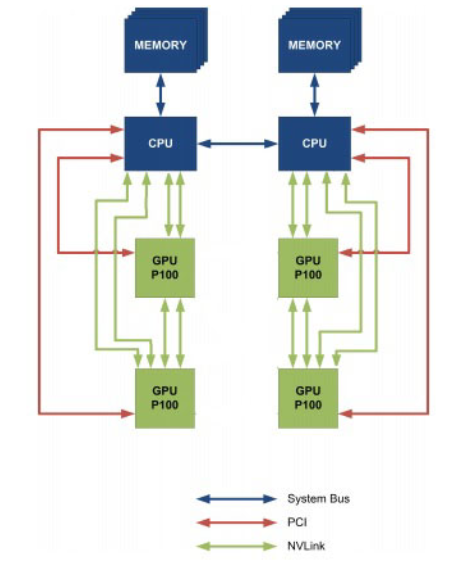
\includegraphics[width=0.8\textwidth]{images/NVLink.png}
                \caption{CPU to GPU and GPU to GPU interconnect using NVLink}
            \end{figure}
    \end{columns}

\end{frame}
\section{Analytic Results}
\subsection{Final Time Distribution}
\begin{frame}
    \frametitle{Analytic Results - de Sitter Expansion}

    de Sitter expansion: $a(t) = e^{-t/t_s}$
    \begin{columns}
        \begin{column}{.5\textwidth}
            \vspace{-0.5in}
            \begin{itemize}
                \item Use Mathematica for simple analytic results
                \item Population distribution highly depends on length of expansion
                \item Population is relatively high for low $k$
                \item Population drops off quickly with $k$
            \end{itemize}
        \end{column}
        \begin{column}{.5\textwidth}
            \begin{figure}[h]
                \centering
                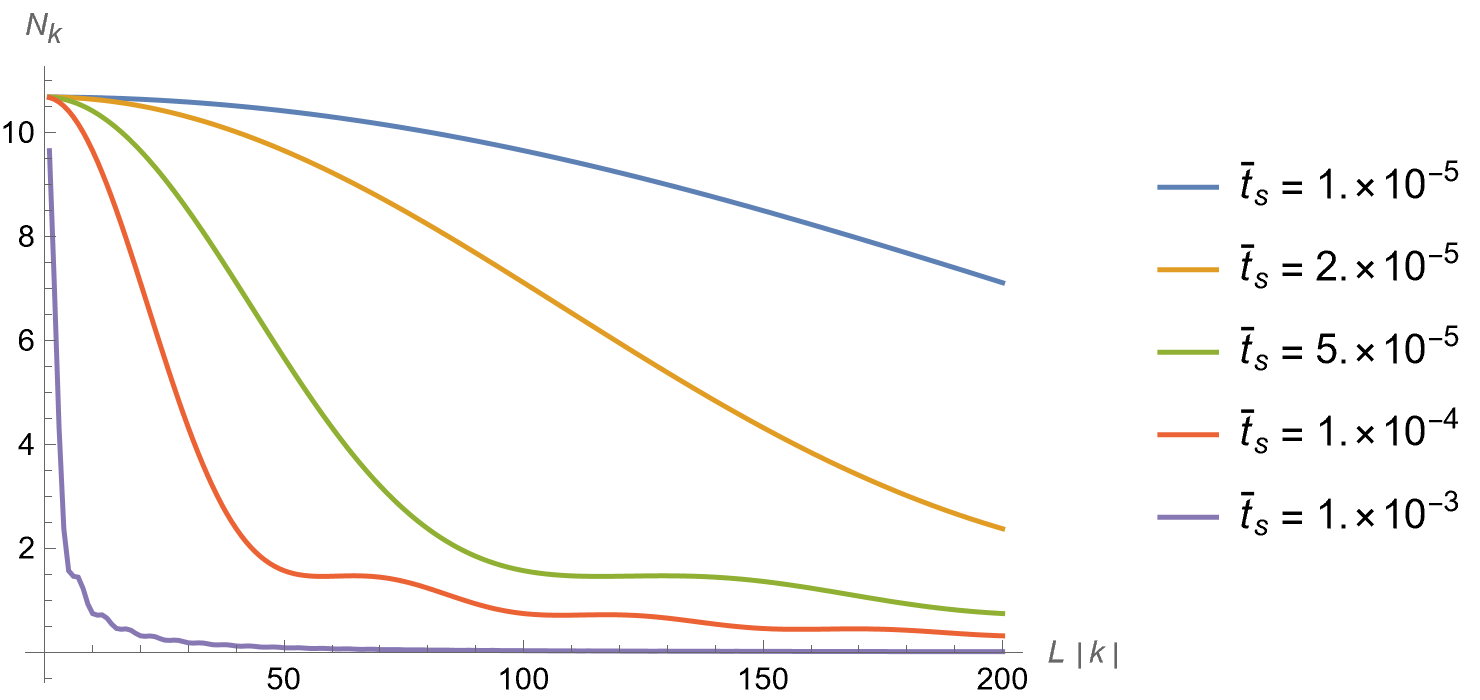
\includegraphics[width=\textwidth]{images/fig2.png}
                \caption{The momentum distribution when the universe stops expanding for multiple effective \\ rates of expansion}
                \label{fig:finalTime}
            \end{figure}
        \end{column}
    \end{columns}
\end{frame}

\subsection{All Time Distribution}
\begin{frame}
    \frametitle{Analytic Results - de Sitter Expansion}

    \begin{figure}[h]
        \centering
        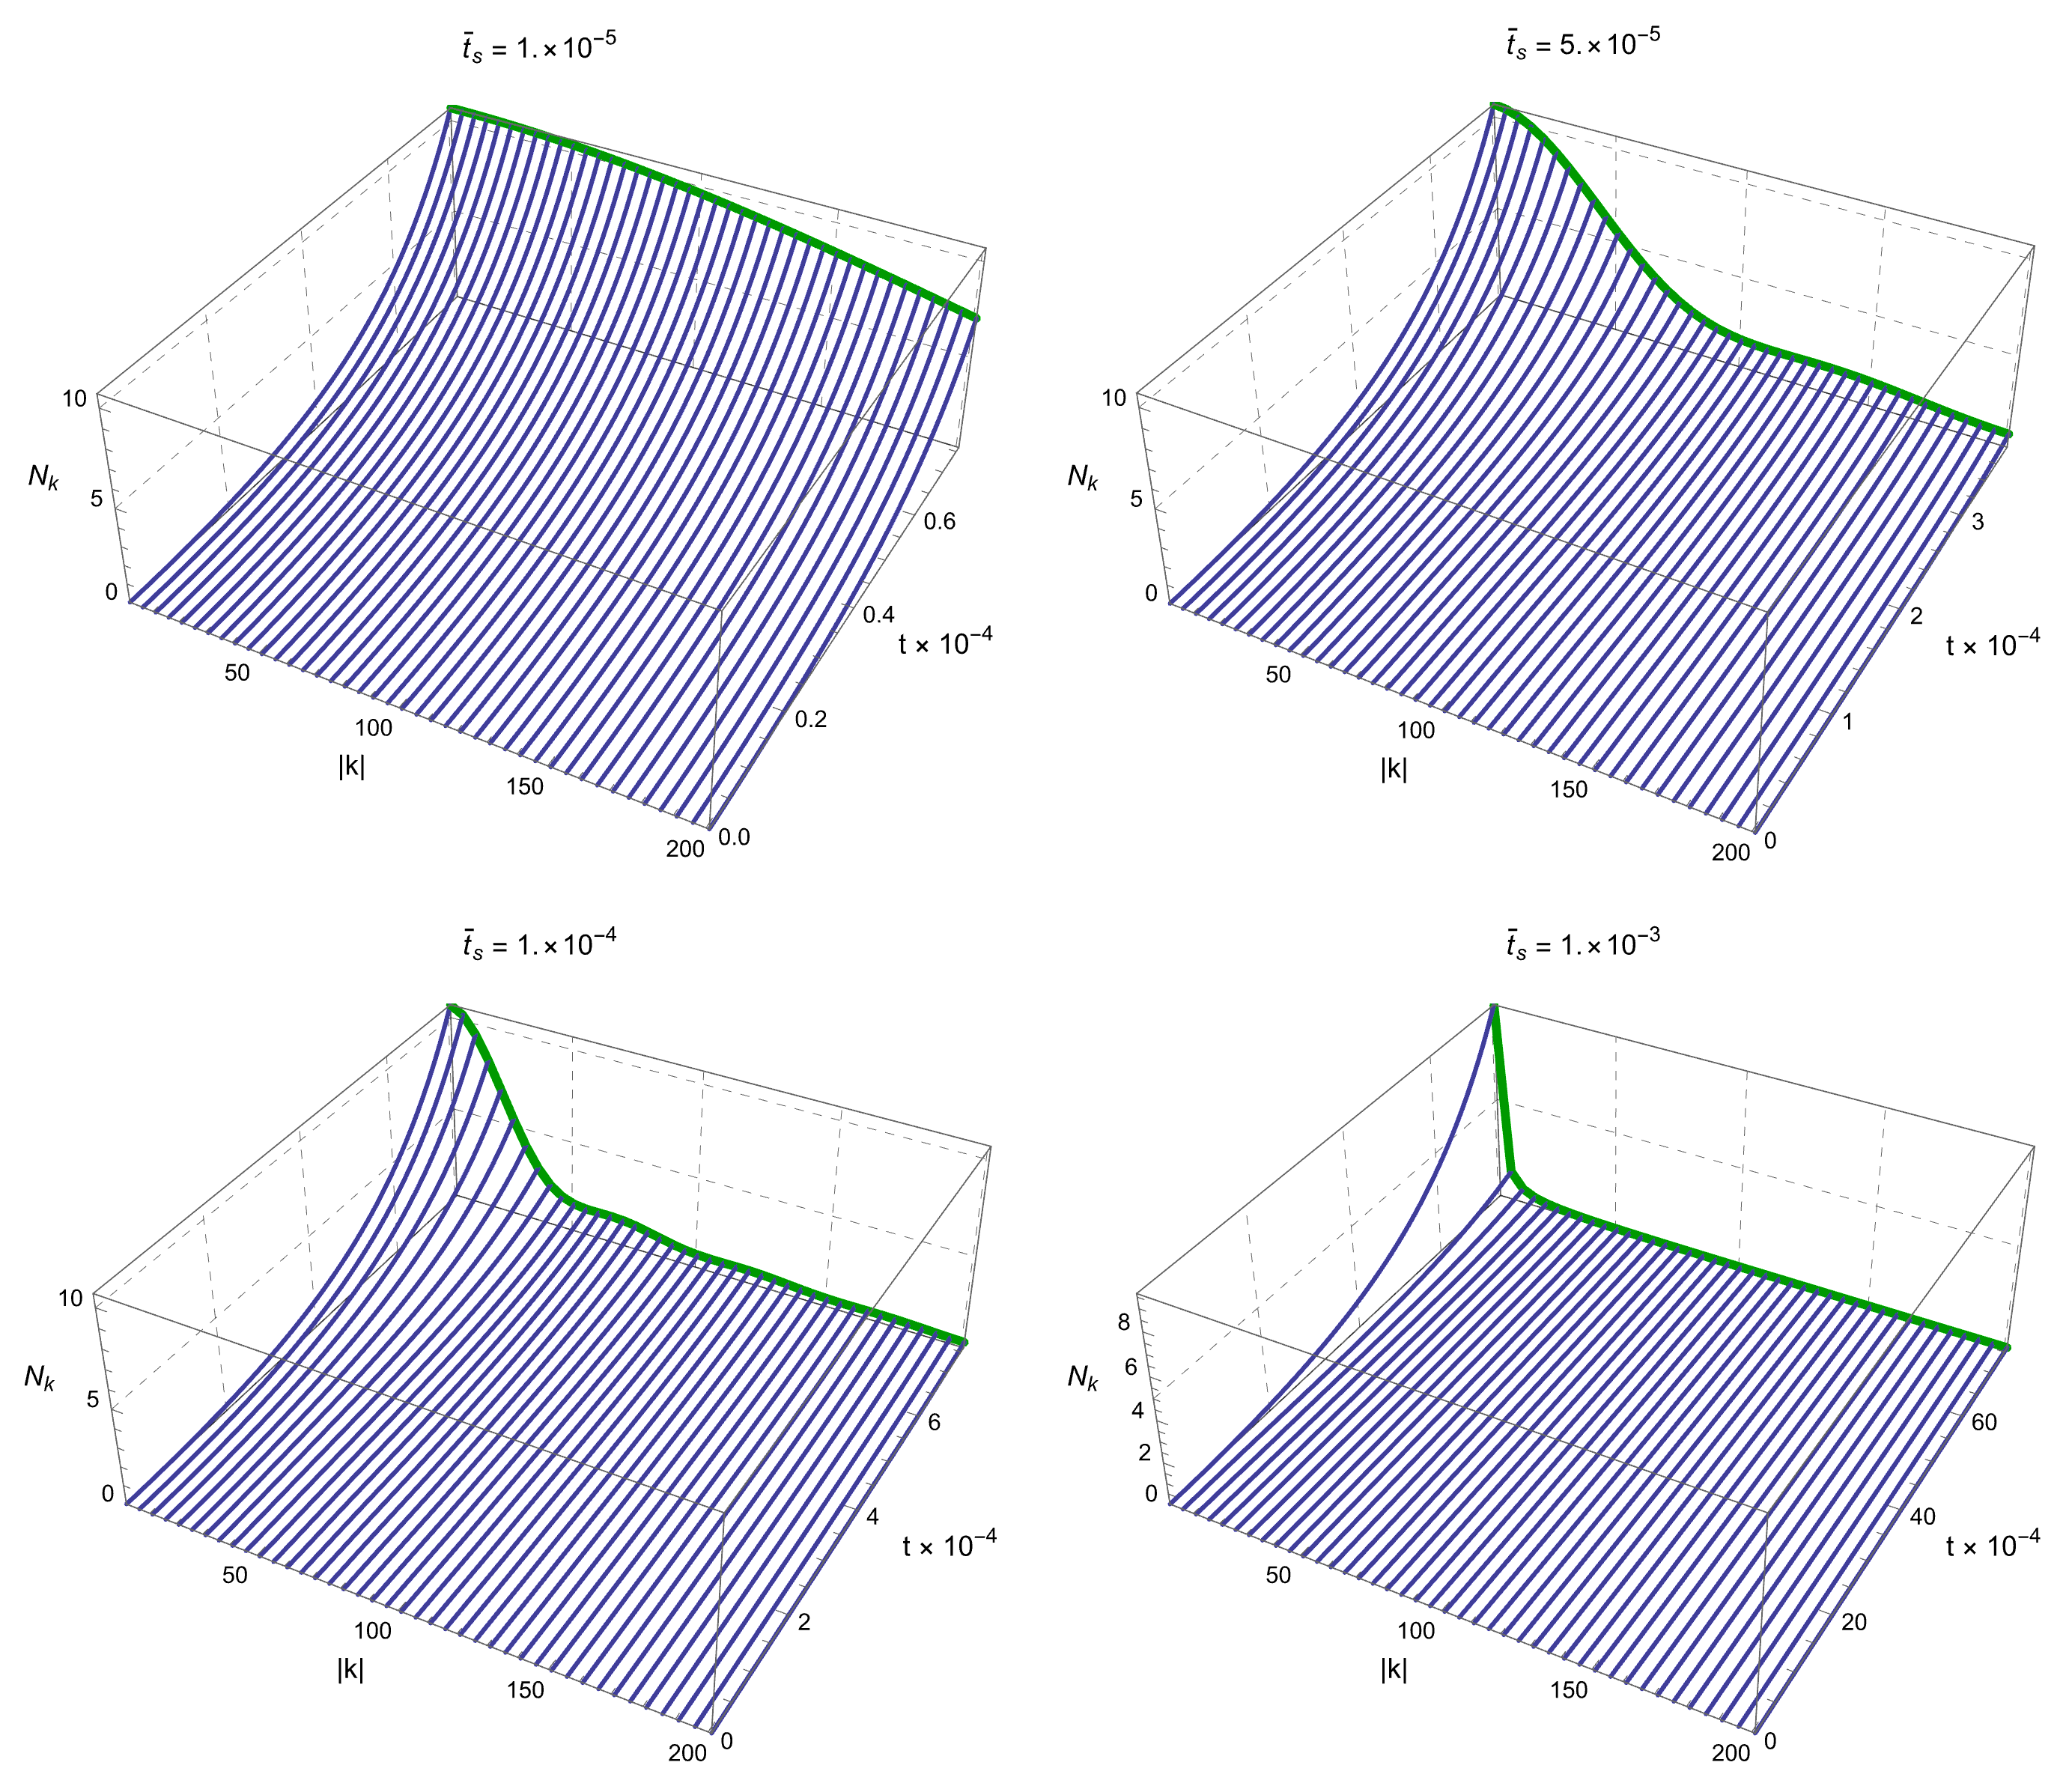
\includegraphics[width=0.5\textwidth]{images/Analytic_Fig_4.png}
        \caption{Momentum distribution throughout the expansion}
        \label{fig:allTime}
    \end{figure}

\end{frame}

\begin{frame}
    \frametitle{Discussion - Why High-Performance Computing?}

    \begin{itemize}
        \item Analytic methods $\implies$ simple expansions
        \item Numeric methods $\implies$ complex expansions
        \item Complex expansions $\implies$ High-performance computational model
    \end{itemize}

\end{frame}

\begin{frame}
    \frametitle{Conclusion}

    \begin{itemize}
        \item A lot of work has been done into the theory of analog universes for different systems
        \item A computational model is needed to provide guidance and support to both theory and experiment
        \item The behavior of particles created from the expansion of the universe is the same as particles in the lab
        \item Need to find the behavior for many different cases
        \item Need to support a general, complex expansion
        \item Use high-performance techniques and hardware for reasonable execution time
    \end{itemize}

\end{frame}

\begin{frame}
    \frametitle{Acknowledgements}

    \begin{itemize}
        \item Dr. Andy Piacsek (CWU)
        \item Dr. Szilard VAJDA (CWU)
        \item Dr. Micheal Braunstein (CWU)
        \item Dr. Brandon Peden (WWU)
    \end{itemize}

\end{frame}

\begin{frame}{Thank you \& Code source}
    \begin{columns}[onlytextwidth]
        \begin{column}{.5\textwidth}
            Thank you for your attention.
            \vspace*{0.1\textheight} \\
            The code for this project is available at:
            \begin{itemize}
                \item GitHub (QR code): \url{github.com/nondairyneutrino/thesis}
                \item My website: \url{nathanwchapman.com}
            \end{itemize}
        \end{column}
        \begin{column}{.5\textwidth}
            \centering
            \qrcode[height=0.67\textheight]{https://github.com/nondairyneutrino/thesis}
        \end{column}
    \end{columns}
    \end{frame}

\begin{frame}[allowframebreaks]
    \frametitle{\bibname}
    \nocite{*}
    \printbibliography
\end{frame}

\end{document}